

\tikzset{every picture/.style={line width=0.75pt}} %set default line width to 0.75pt        

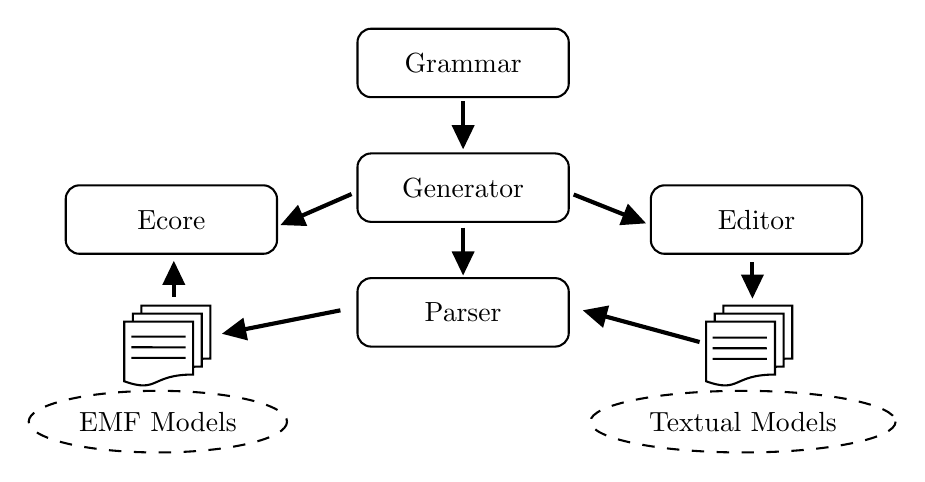
\begin{tikzpicture}[x=0.75pt,y=0.75pt,yscale=-1,xscale=1]
%uncomment if require: \path (0,440); %set diagram left start at 0, and has height of 440

%Rounded Rect [id:dp818707961672321] 
\draw  [fill={rgb, 255:red, 255; green, 255; blue, 255 }  ,fill opacity=1 ] (185.16,18.8) .. controls (185.16,15.16) and (188.11,12.21) .. (191.75,12.21) -- (280.36,12.21) .. controls (284,12.21) and (286.96,15.16) .. (286.96,18.8) -- (286.96,38.59) .. controls (286.96,42.23) and (284,45.19) .. (280.36,45.19) -- (191.75,45.19) .. controls (188.11,45.19) and (185.16,42.23) .. (185.16,38.59) -- cycle ;
%Rounded Rect [id:dp5004620289072519] 
\draw  [fill={rgb, 255:red, 255; green, 255; blue, 255 }  ,fill opacity=1 ] (326.5,94.26) .. controls (326.5,90.62) and (329.45,87.67) .. (333.1,87.67) -- (421.7,87.67) .. controls (425.35,87.67) and (428.3,90.62) .. (428.3,94.26) -- (428.3,114.05) .. controls (428.3,117.69) and (425.35,120.65) .. (421.7,120.65) -- (333.1,120.65) .. controls (329.45,120.65) and (326.5,117.69) .. (326.5,114.05) -- cycle ;
%Rounded Rect [id:dp4485202200852796] 
\draw  [fill={rgb, 255:red, 255; green, 255; blue, 255 }  ,fill opacity=1 ] (185.16,78.89) .. controls (185.16,75.25) and (188.11,72.3) .. (191.75,72.3) -- (280.36,72.3) .. controls (284,72.3) and (286.96,75.25) .. (286.96,78.89) -- (286.96,98.68) .. controls (286.96,102.32) and (284,105.27) .. (280.36,105.27) -- (191.75,105.27) .. controls (188.11,105.27) and (185.16,102.32) .. (185.16,98.68) -- cycle ;
%Rounded Rect [id:dp34928126985064645] 
\draw  [fill={rgb, 255:red, 255; green, 255; blue, 255 }  ,fill opacity=1 ] (44.59,94.26) .. controls (44.59,90.62) and (47.55,87.67) .. (51.19,87.67) -- (139.8,87.67) .. controls (143.44,87.67) and (146.39,90.62) .. (146.39,94.26) -- (146.39,114.05) .. controls (146.39,117.69) and (143.44,120.65) .. (139.8,120.65) -- (51.19,120.65) .. controls (47.55,120.65) and (44.59,117.69) .. (44.59,114.05) -- cycle ;
%Rounded Rect [id:dp899217105871126] 
\draw  [fill={rgb, 255:red, 255; green, 255; blue, 255 }  ,fill opacity=1 ] (185.16,138.98) .. controls (185.16,135.34) and (188.11,132.38) .. (191.75,132.38) -- (280.36,132.38) .. controls (284,132.38) and (286.96,135.34) .. (286.96,138.98) -- (286.96,158.77) .. controls (286.96,162.41) and (284,165.36) .. (280.36,165.36) -- (191.75,165.36) .. controls (188.11,165.36) and (185.16,162.41) .. (185.16,158.77) -- cycle ;
%Flowchart: Multidocument [id:dp814245162277164] 
\draw  [fill={rgb, 255:red, 255; green, 255; blue, 255 }  ,fill opacity=1 ] (81.08,145.66) -- (114.29,145.66) -- (114.29,171.11) .. controls (93.54,171.11) and (97.69,180.29) .. (81.08,174.35) -- cycle ; \draw  [fill={rgb, 255:red, 255; green, 255; blue, 255 }  ,fill opacity=1 ] (76.93,149.52) -- (110.14,149.52) -- (110.14,174.97) .. controls (89.39,174.97) and (93.54,184.15) .. (76.93,178.21) -- cycle ; \draw  [fill={rgb, 255:red, 255; green, 255; blue, 255 }  ,fill opacity=1 ] (72.78,153.37) -- (105.99,153.37) -- (105.99,178.83) .. controls (85.24,178.83) and (89.39,188.01) .. (72.78,182.07) -- cycle ;
%Straight Lines [id:da659202853659377] 
\draw [fill={rgb, 255:red, 255; green, 255; blue, 255 }  ,fill opacity=1 ]   (76.2,160.56) -- (102.38,160.59) ;
%Straight Lines [id:da8271632436642871] 
\draw [fill={rgb, 255:red, 255; green, 255; blue, 255 }  ,fill opacity=1 ]   (76.2,165.69) -- (102.38,165.71) ;
%Straight Lines [id:da22701123408508272] 
\draw [fill={rgb, 255:red, 255; green, 255; blue, 255 }  ,fill opacity=1 ]   (76.2,170.81) -- (102.38,170.83) ;


%Flowchart: Multidocument [id:dp49717070559395604] 
\draw  [fill={rgb, 255:red, 255; green, 255; blue, 255 }  ,fill opacity=1 ] (361.43,145.66) -- (394.63,145.66) -- (394.63,171.11) .. controls (373.88,171.11) and (378.03,180.29) .. (361.43,174.35) -- cycle ; \draw  [fill={rgb, 255:red, 255; green, 255; blue, 255 }  ,fill opacity=1 ] (357.28,149.52) -- (390.48,149.52) -- (390.48,174.97) .. controls (369.73,174.97) and (373.88,184.15) .. (357.28,178.21) -- cycle ; \draw  [fill={rgb, 255:red, 255; green, 255; blue, 255 }  ,fill opacity=1 ] (353.12,153.37) -- (386.33,153.37) -- (386.33,178.83) .. controls (365.58,178.83) and (369.73,188.01) .. (353.12,182.07) -- cycle ;
%Straight Lines [id:da5642847406466045] 
\draw [fill={rgb, 255:red, 255; green, 255; blue, 255 }  ,fill opacity=1 ]   (356.28,161.03) -- (382.46,161.05) ;
%Straight Lines [id:da9779186616916171] 
\draw [fill={rgb, 255:red, 255; green, 255; blue, 255 }  ,fill opacity=1 ]   (356.28,166.15) -- (382.46,166.18) ;
%Straight Lines [id:da8217185402464098] 
\draw [fill={rgb, 255:red, 255; green, 255; blue, 255 }  ,fill opacity=1 ]   (356.28,171.28) -- (382.46,171.3) ;


%Straight Lines [id:da4555835119587406] 
\draw [fill={rgb, 255:red, 255; green, 255; blue, 255 }  ,fill opacity=1 ][line width=1.5]    (236.06,47.21) -- (236.06,66.27) ;
\draw [shift={(236.06,70.27)}, rotate = 270] [fill={rgb, 255:red, 0; green, 0; blue, 0 }  ][line width=0.08]  [draw opacity=0] (11.61,-5.58) -- (0,0) -- (11.61,5.58) -- cycle    ;
%Straight Lines [id:da2586670416419199] 
\draw [fill={rgb, 255:red, 255; green, 255; blue, 255 }  ,fill opacity=1 ][line width=1.5]    (236.06,108) -- (236.06,127.06) ;
\draw [shift={(236.06,131.06)}, rotate = 270] [fill={rgb, 255:red, 0; green, 0; blue, 0 }  ][line width=0.08]  [draw opacity=0] (11.61,-5.58) -- (0,0) -- (11.61,5.58) -- cycle    ;
%Straight Lines [id:da2552674310073062] 
\draw [fill={rgb, 255:red, 255; green, 255; blue, 255 }  ,fill opacity=1 ][line width=1.5]    (182.3,91.87) -- (151.77,105.18) ;
\draw [shift={(148.1,106.78)}, rotate = 336.45] [fill={rgb, 255:red, 0; green, 0; blue, 0 }  ][line width=0.08]  [draw opacity=0] (11.61,-5.58) -- (0,0) -- (11.61,5.58) -- cycle    ;
%Straight Lines [id:da29550662771480396] 
\draw [fill={rgb, 255:red, 255; green, 255; blue, 255 }  ,fill opacity=1 ][line width=1.5]    (320.43,104.49) -- (289.32,92.1) ;
\draw [shift={(324.15,105.97)}, rotate = 201.71] [fill={rgb, 255:red, 0; green, 0; blue, 0 }  ][line width=0.08]  [draw opacity=0] (11.61,-5.58) -- (0,0) -- (11.61,5.58) -- cycle    ;
%Straight Lines [id:da3813677861719633] 
\draw [fill={rgb, 255:red, 255; green, 255; blue, 255 }  ,fill opacity=1 ][line width=1.5]    (375.44,124.77) -- (375.44,138.24) ;
\draw [shift={(375.44,142.24)}, rotate = 270] [fill={rgb, 255:red, 0; green, 0; blue, 0 }  ][line width=0.08]  [draw opacity=0] (11.61,-5.58) -- (0,0) -- (11.61,5.58) -- cycle    ;
%Straight Lines [id:da3940907258410822] 
\draw [fill={rgb, 255:red, 255; green, 255; blue, 255 }  ,fill opacity=1 ][line width=1.5]    (96.67,128.07) -- (96.67,141.54) ;
\draw [shift={(96.67,124.07)}, rotate = 90] [fill={rgb, 255:red, 0; green, 0; blue, 0 }  ][line width=0.08]  [draw opacity=0] (11.61,-5.58) -- (0,0) -- (11.61,5.58) -- cycle    ;
%Straight Lines [id:da3280771928101003] 
\draw [fill={rgb, 255:red, 255; green, 255; blue, 255 }  ,fill opacity=1 ][line width=1.5]    (176.93,147.89) -- (123.84,158.4) ;
\draw [shift={(119.91,159.18)}, rotate = 348.81] [fill={rgb, 255:red, 0; green, 0; blue, 0 }  ][line width=0.08]  [draw opacity=0] (11.61,-5.58) -- (0,0) -- (11.61,5.58) -- cycle    ;
%Straight Lines [id:da9478402467031726] 
\draw [fill={rgb, 255:red, 255; green, 255; blue, 255 }  ,fill opacity=1 ][line width=1.5]    (349.99,163.16) -- (297.62,148.94) ;
\draw [shift={(293.75,147.89)}, rotate = 375.19] [fill={rgb, 255:red, 0; green, 0; blue, 0 }  ][line width=0.08]  [draw opacity=0] (11.61,-5.58) -- (0,0) -- (11.61,5.58) -- cycle    ;

% Text Node
\draw  [fill={rgb, 255:red, 255; green, 255; blue, 255 }  ,fill opacity=1 ][dash pattern={on 4.5pt off 4.5pt}]  (88.99, 201.52) circle [x radius= 62.23, y radius= 14.85]   ;
\draw (88.99,201.52) node   [align=left] {EMF Models};
% Text Node
\draw  [fill={rgb, 255:red, 255; green, 255; blue, 255 }  ,fill opacity=1 ][dash pattern={on 4.5pt off 4.5pt}]  (370.9, 201.52) circle [x radius= 73.54, y radius= 14.85]   ;
\draw (370.9,201.52) node   [align=left] {Textual Models};
% Text Node
\draw (236.06,148.87) node   [align=left] {Parser};
% Text Node
\draw (377.4,104.16) node   [align=left] {Editor};
% Text Node
\draw (236.06,28.7) node   [align=left] {Grammar};
% Text Node
\draw (95.49,104.16) node   [align=left] {Ecore};
% Text Node
\draw (236.06,88.79) node   [align=left] {Generator};


\end{tikzpicture}
